\chapter{Notes 
%\small{\textit{-- Team-11}} 
\index{Chapter!Notes }
\index{Notes}
\label{Chapter::Notes}}\
\section{Mission Statement \label{Section::Mission Statement} }
The primary purpose of this project is to protect stakeholders from falling victim to deceptive clauses in contracts that may undermine their best interests, either intentionally or unintentionally or via other disruptive means. These clauses could cause harm to the signing party through various means, such as monetary loss or other negative consequences that may impact the livelihood of the concerned stakeholder as a whole. 

\section{Key Stakeholders \label{Section::Key Stakeholders} }
The key stakeholders for our project are as follows: 
\begin{itemize}
    \item Direct daily consumers: Direct daily customers are individuals who want to protect themselves against being misled by fraudulent companies. By identifying potentially fraudulent phrases in contracts, Clauseguard adds an extra degree of security for these clients. Direct daily clients who utilize Clauseguard can be secure that they are getting fair deals and can stay out of trouble by doing so.
    \item Commercial enterprises: Clauseguard is a tool that commercial enterprises can employ to shield themselves from any legal responsibilities. Enterprises can find and remove potentially fraudulent clauses from their contracts by analyzing them using natural language processing tools. This can assist them in adhering to the law and ensuring that they are not taking part in any fraudulent activity.
    \item Criminal lawyers: As part of their legal investigations, criminal attorneys might use Clauseguard to find fraudulent clauses in contracts. Criminal attorneys can find probable fraud evidence in contracts by employing natural language processing tools to analyze contracts. This information can then be utilized to support a case against dishonest businesses.
    \item Law enforcement: Clauseguard can be used by law enforcement organizations to find possibly fraudulent activity taking place within businesses. Law enforcement organizations can find potential fraud evidence through the analysis of contracts, which can then be utilized to support a case against dishonest businesses. This can ensure that firms run fairly and transparently and protect consumers.
\end{itemize}




\section{Key Drivers \label{Section::Key Drivers} }
The key drivers for our project ClauseGuard are as follows: 
\begin{itemize}
    \item Data Availability: A large dataset of already available online documents helped bring this project to fruition. Although a large dataset is present, the average person would need extensive knowledge in legal studies to understand the implications of it. 
    \item Emotional Motivations: Our team was motivated to select this project based on personal experiences that we faced. Several of our friends and family members have previously fallen victim to deceptive contractual terms leading to significant hardships and losses in physical, financial and mental areas. 
    \item Changing Legal Landscape: In today's fast-paced and dynamic legal landscape, laws and regulations are subject to frequent updates and revisions. These changes have a direct impact on businesses, individuals, and content creators, making it imperative for them to stay informed and compliant.

A prime example of such legal regulatory changes is the introduction of bill C-11 in Canada. This legislation imposes new obligations and responsibilities on content creators, emphasizing the importance of careful consideration regarding the content they produce and publish. The implementation of this bill necessitates a comprehensive understanding of the legal requirements and potential implications, compelling creators to seek reliable tools and resources that can assist them in navigating these complexities. 
Such legal changes drive the need for a software like ClauseGuard. Its sophisticated capabilities enable users to effectively analyze and assess their contracts, identifying any deceptive or unclear clauses that may not align with the evolving legal landscape thereby preventing years of physical, financial and mental hardships.

\item Growing Need for Transparency and Fairness: There is a growing demand for greater transparency and fairness in legal agreements. By identifying potentially fraudulent or misleading clauses, the ClauseGuard system can help to increase transparency and fairness in contracts.

\item Lack of Accessible Legal Expertise: Not everyone has access to legal expertise to review contracts, which can leave individuals and small businesses particularly vulnerable to fraudulent clauses. ClauseGuard provides an accessible solution to this problem by leveraging AI to analyze contracts.
\end{itemize}



\section{Key Constraints \label{Section::Key Constraints} }

\begin{itemize}
    \item Data Privacy and Security: The ClauseGuard system will be dealing with potentially sensitive and confidential documents. It is crucial that the system maintains the privacy and security of these documents, ensuring that the data is not misused or accessed by unauthorized individuals.
    \item Expert Input for Model Training: The ClauseGuard model needs to be trained based on the input of legal experts to ensure it correctly identifies fraudulent clauses. However, scheduling interviews and obtaining extensive legal input from lawyers or paralegals is a significant challenge, especially without networking or financial resources and one we've not been able to schedule despite numerous attempts.
    \item Variations in Legal Document Structures: The system must be capable of handling contracts that are written in different terminologies and structures, as legal documents can vary significantly across countries and regions. This adds a layer of complexity to the task of creating a universally applicable model.
    \item Legal and Regulatory Compliance: Operating in the legal domain, ClauseGuard must comply with all relevant laws and regulations. This includes data protection laws and potentially also laws related to the provision of legal advice.
    \item Resource Limitations: The development of ClauseGuard, requires significant resources, including skilled personnel, computational power, and time. These resources may limit the scope and speed of development.
    \item  Transparency and Explainability: In addition to identifying potentially fraudulent clauses, the system must provide understandable explanations for its decisions. This requirement for transparency and explainability can add complexity to the model development process.
    \end{itemize}

\section{Key Requirements \label{Section::Key Requirements}}

\begin{itemize}
    \item User Requirements: Some of the user Requirements that we've identified when conducting interviews are given below: 
    \begin{itemize}
        \item The model must be encapsulated within a website format, ensuring its accessibility across various platforms and devices. This ensures universal access irrespective of the user's choice of hardware or operating system and ensures access to anyone irrespective of their current geographic location. 
        \item The model must demonstrate high accuracy and precision in identifying harmful clauses, with a particular focus on minimizing false positives. This is to ensure that users can trust the system's alerts and do not waste time investigating harmless clauses flagged erroneously.
        \item  The model must not only flag potentially harmful clauses but also provide a clear, concise, and understandable explanation for why a particular clause has been flagged. This will foster trust in the system and enable users to make informed decisions based on its output.
        \item The model must be robust enough to handle complex documents of varying lengths. It should be designed to analyze and flag harmful clauses in both short and lengthy documents, ensuring it caters to a wide range of contract types.
        \item The model must be regularly updated to keep pace with the evolving legal landscape. These updates should reflect changes in legal standards, emerging contract trends, and user feedback.
        \item The model must support documents in various formats, such as PDF, LaTeX, Word, etc. This ensures that users can analyze contracts in their original format without the need for time-consuming conversions.


        













    \end{itemize}
    \item Business Requirements: 
    \begin{itemize}
        \item The model must adhere to all relevant legal systems and regulatory bodies. This extends to maintaining compliance with laws and regulations related to confidential data. As laws vary globally, the model must have the capacity to adapt and adjust to diverse legal environments and requirements.
        \item The model should be designed with a flexible and robust Application Programming Interface (API) to facilitate seamless integration with various systems used across the industry. This would ensure that the model can be smoothly incorporated into existing infrastructures, enhancing its utility and accessibility.
        \item The model must be equipped with robust security measures to protect against data breaches and security leaks. We've identified that leveraging cloud-based infrastructure systems such as Amazon Web Services (AWS), along with their key management services, will provide a robust security framework for the system.
        \item Beyond explaining why certain clauses are flagged, the model should offer an option for a more technical breakdown of its decision-making process. This interpretability feature would be particularly useful for legal experts and system administrators seeking to understand the underlying mechanics of the model's decisions.
        \item The model should be equipped to handle batch processing of multiple contracts at once. This feature would be crucial for businesses or legal entities dealing with a large volume of contracts.
        \item The system should be capable of extracting and managing relevant metadata from the contracts, such as dates, involved parties, and contract types. This would support advanced analysis and tracking of contract features over time.
        \item The system should be capable of extracting and managing relevant metadata from the contracts, such as dates, involved parties, and contract types. This would support advanced analysis and tracking of contract features over time.














    \end{itemize}
    \item Systems Requirements: 
    \begin{itemize}
        \item The system will incorporate automated monitoring tools to alert administrators about any performance issues, potential system failures, or security threats. Coverity is one such tool that can quickly identify any defects in code and suggest improvements to fix those defects. 
        \item While the system will support documents in varying formats such as PDF, Word, and LaTeX, it must also be capable of handling other less common but industry-relevant formats, like RTF.
        \item The system must have the ability to handle variable load patterns effectively. This includes peak periods when there might be a surge in the number of contracts being uploaded for review. This can be achieved by the introduction of load balancers.
        \item The system shall efficiently manage computational resources, ensuring optimal utilization of available resources even during peak load times.
        \item The system must be designed to handle potential future data migration or system upgrades without significant downtime or data loss. This can be achieved by using A centralized backup system such as Velero which can be used as a data migration tool and recovery in case of a primary system failure. 










    \end{itemize}
    \item Security Requirements: 
    \begin{itemize}
        \item The system must implement RBAC ( Role-Based Access Control) or IAM( Identity Access Management) when leverage AWS services, allowing system administrators to define roles and permissions, ensuring that only authorized individuals have access to certain functionalities such as cloud infrastructure, model development, database access etc. 
        \item The system must ensure that the model training process itself does not introduce any vulnerability that could be exploited by reverse engineering a legacy version of the model. 
        \item An intrusion detection system will be integrated to monitor and alert for any potential security threats or breaches in real-time.
        \item The system must implement a stringent data retention policy, where uploaded contracts are not stored beyond the necessary time frame required for analysis.
        \item Any APIs used or exposed by the system are required to be designed with best security practices to prevent unauthorized access or data leaks.
        \item The system shall implement two-factor authentication for user logins.












    \end{itemize}
    \item Quality Requirements: 
    \begin{itemize}
        \item The system must continuously track the model’s performance metrics against predefined benchmarks to ensure consistent quality of analysis.
        \item Beyond simple textual analysis, the system should ensure contextual accuracy, recognizing that the same phrase might have different implications in different types of contracts.
        \item The system must yield consistent results when analyzing the same contract or similar clauses multiple times.
        \item The system shall have a mechanism for users to provide feedback on the system's performance and accuracy, facilitating continuous improvement.
        \item The system's outputs (e.g., flagged clauses, risk scores) must be communicated clearly and concisely, using non-technical language that can be easily understood by users without a legal or technical background.













    \end{itemize}
\end{itemize}



\section{Requirements Elicitation Process \label{Section::Requirements Elicitation Process} }
For the interviews, we decided to use the following elicitation techniques: 
\begin{itemize}
    \item Brainstorming: We held informal meetings with the potential stakeholders and conducted interviews asking informal questions. 
    \item Questionnaires: We have developed surveys on how the system should operate and the features they would like to see. We have yet to share the surveys as we are finalizing the questions that we want to ask.  
    \item User stories: We asked potential stakeholders to share their personal experiences with being deceived by fraudulent contract clauses. We also sought their insight on how our system could help prevent them from falling victim to similar deceptive clauses in the future
\end{itemize}


\section{ Requirement Validation and Analysis \label{Section::Requirement Validation and Analysis} }
The requirements validation and analysis for ClauseGuard is as follows: 
\begin{itemize}
    \item First we developed a simplified prototype of the system to demonstrate the working of the system. Then we confirmed the requirements from the stakeholders where they were accurate or not. 
    \item We used task analysis in order to check the the model is performing in accordance with the user stories laid out by the stakeholders. 
    \item Thirdly, we elicited and considered the different viewpoints from the stakeholders in order to resolve any conflicts. One example was that some stakeholders wanted an explanation of why the a particular clause was flagged however, it was not a requirement for other stakeholders who mentioned that they may not have the time to read through an explanation and just the risk indicator was enough. 
    \item For analysis, we made sure to use imperatives while describing the requirements and during the creation of this ConOps document. imperatives such as Shall, must, will are used extensively throughout the document. 
    \end{itemize}

    
\section{ User Interviews \label{Section::User Interviews} }
We conducted user interviews with the following stakeholders. We used brainstorming, user stories and questionnaires to elicit requirements from the users which is highlighted below: 

\begin{itemize}
\item Date Conducted: 04/21/2023
\item Place: In-person
    \item Full Name: Hrishikesh Kathikar

    \item Age: 22

    \item Profession:Student 

    \item Email:hakathikar@gmail.com

    \item Question Asked : What kind of information would you like to see in terms and conditions to help you make a more informed decision?

    \item Answer: highlighted information regarding privacy violations, information summarized in fewer points
\end{itemize}
\begin{itemize}
\item Date Conducted: 04/22/2023
\item Place: In-person
    \item Full Name: Sai satvika

    \item Age: 20

    \item Profession:Student 

    \item Email:satvikakongara@gmail.com

    \item Question Asked : Do you think that companies should be required to use plain language in their terms and conditions?

    \item Answer:Yes 
\end{itemize}



\begin{itemize}
\item Date Conducted: 04/18/2023
\item Place: In-person
    \item Full Name: Mythri Shivakumar

    \item Age: 22

    \item Profession:Software Development Engineer 

    \item Email:geetamythri27@gmail.com

    \item Question Asked : Have you ever been in a situation where you felt like you were taken advantage of because of a clause in a contract?

    \item Answer: Yes, plenty of times 
\end{itemize}
\begin{itemize}
\item Date Conducted: 04/25/2023
\item Place: In-person
    \item Full Name: Yashwanth Vuppula  

    \item Age: 19

    \item Profession:Student 

    \item Email:yashwanthvuppula88@gmail.com

    \item Question Asked : How do you think that a tool like Clauseguard could benefit you personally?

    \item Answer: Would make it easier for me to sign up more.
\end{itemize}
\begin{itemize}
\item Date Conducted: 04/24/2023
\item Place: Online
    \item Full Name: Shubham Raj

    \item Age: 21

    \item Profession:Unity Programmer 

    \item Email:shubhamraj2001@gmail.com

    \item Question Asked : Do you regularly register or sign up for applications and websites?

    \item Answer: yes

    \item Question: If yes, on a scale one to 10 how often do you register
    \item Answer: 10

    \item Question: What kind of information would you like to see in terms and conditions to help you make a more informed decision?

    \item Answer: Data collection, my account details and photos won't be used after I deactivate my account

    \item Question: Do you think that companies should be required to use plain language in their terms and conditions?

    \item Answer: Yes, so that its easy for every individual to understand. 

    \item Question: Would you be willing to pay a fee to use a tool like Clauseguard to help protect yourself from fraudulent clauses?

    \item Answer: Yes because it will help me saving a lot of money later down the line. 

    \item Question: Have you ever been in a situation where you felt like you were taken advantage of because of a clause in a contract?

    \item Answer: Yes

    \item Question: How do you think that a tool like Clauseguard could benefit you personally?

    \item Answer: It will help me make informed decisions and help me not sign up for applications that would otherwise waste my time. 

    \item Question: Do you think that companies intentionally include fraudulent clauses in their contracts, or is it usually just a mistake?

    \item Answer: Yes, they include fraud clauses intentionally so that they cant be held liable for any wrongdoings. 

    \item Question: How do you think that awareness of fraudulent clauses can be increased among the general public?

    \item Answer: By educating the public via news, podcasts, seminars, workshops

    \item Question: Have you ever heard of any companies that are particularly notorious for including fraudulent clauses in their contracts?

    \item Answer: Yes, Meta, Match.com

    \item Question: How confident do you feel in your ability to detect fraudulent clauses in a contract on your own?

    \item Answer: Not at all confident 

    
\end{itemize}


\begin{itemize}
\item Date Conducted: 04/27/2023
\item Place: In-person
    \item Full Name: Sameer Kaza

    \item Age: 31

    \item Profession: Senior Medical Engineering Specialist  

    \item Email:Kzsam90@gmail.com

    \item Question Asked : Do you regularly register or sign up for applications and websites?

    \item Answer: NO

    \item Question: If yes, on a scale one to 10 how often do you register
    \item Answer: NO

    \item Question: What kind of information would you like to see in terms and conditions to help you make a more informed decision?

    \item Answer: I would like to see the terms and conditions be summarized at the top

    \item Question: Do you think that companies should be required to use plain language in their terms and conditions?

    \item Answer: Yes 

    \item Question: Would you be willing to pay a fee to use a tool like Clauseguard to help protect yourself from fraudulent clauses?

    \item Answer: Yes

    \item Question: Have you ever been in a situation where you felt like you were taken advantage of because of a clause in a contract?

    \item Answer: No

    \item Question: How do you think that a tool like Clauseguard could benefit you personally?

    \item Answer: Would make it easier for me to sign up more

    \item Question: Do you think that companies intentionally include fraudulent clauses in their contracts, or is it usually just a mistake?

    \item Answer: Not sure

    \item Question: How do you think that awareness of fraudulent clauses can be increased among the general public?

    \item Answer: By including the fraudulent history cases in the forms

    \item Question: Have you ever heard of any companies that are particularly notorious for including fraudulent clauses in their contracts?

    \item Answer: Cable companies

    \item Question: How confident do you feel in your ability to detect fraudulent clauses in a contract on your own?

    \item Answer: Pretty good


    \end{itemize}

\begin{figure}[H]
    \centering
    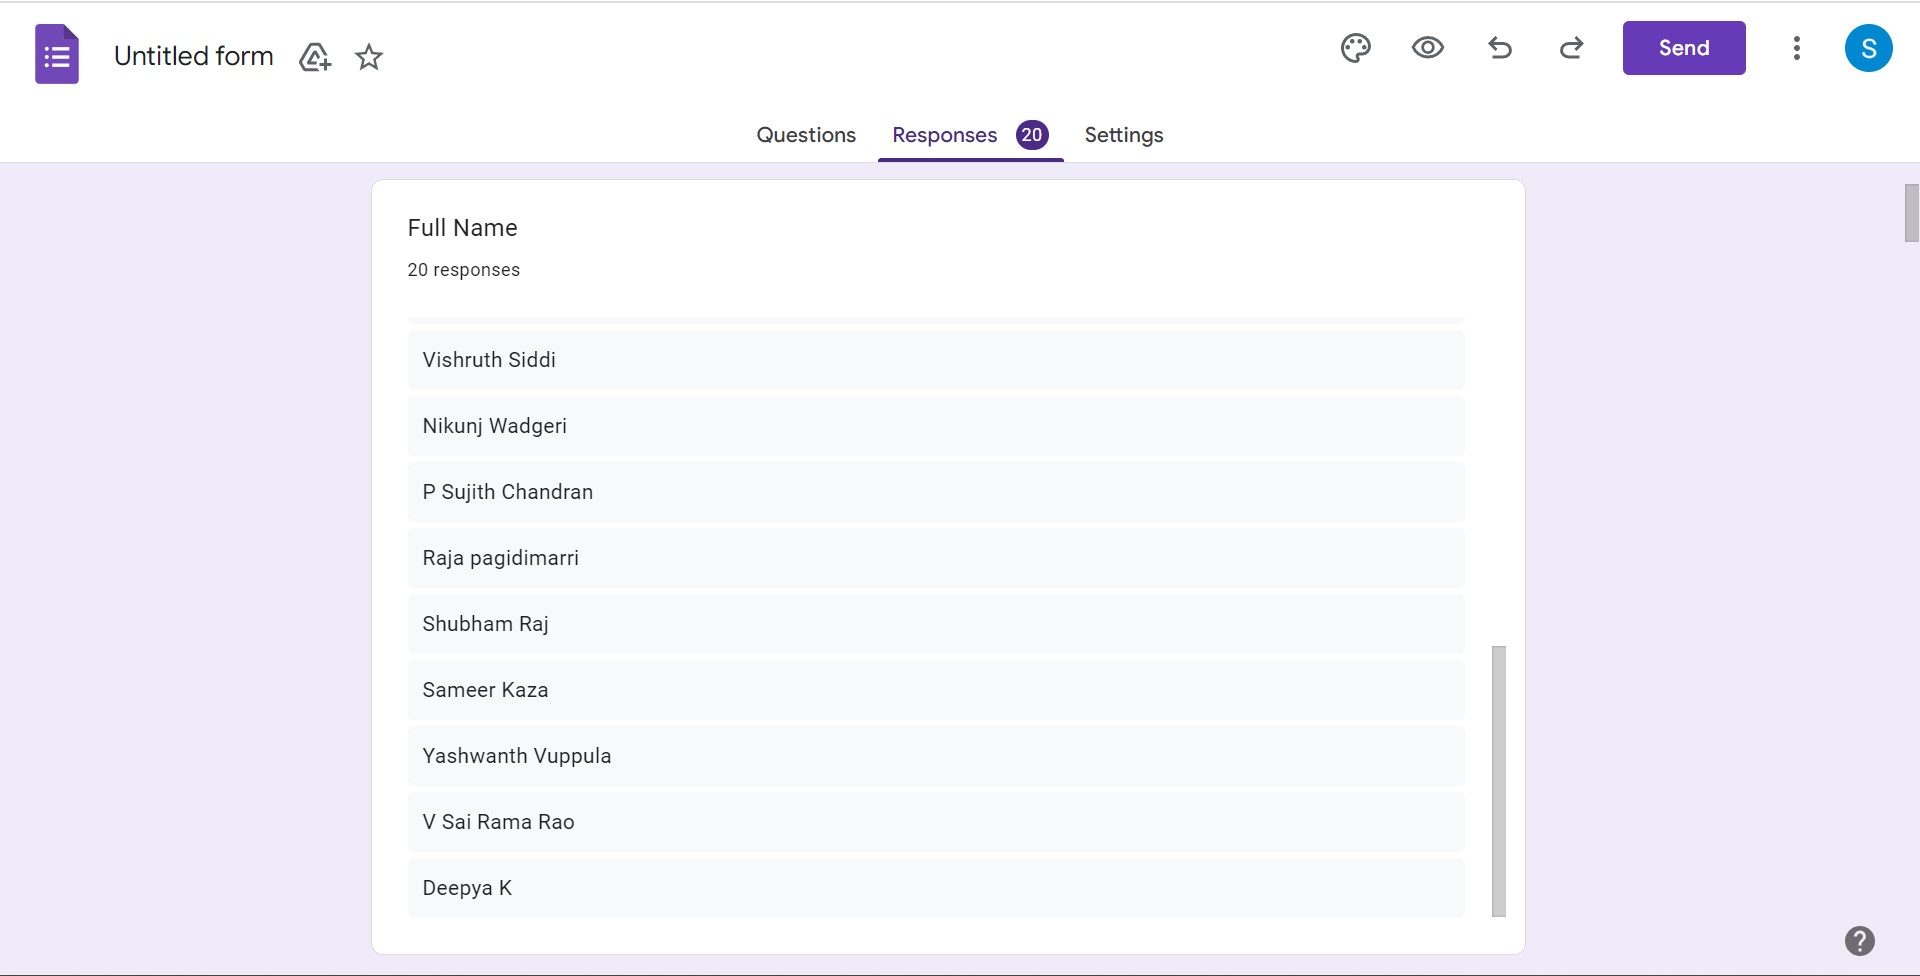
\includegraphics[scale=0.43]{Figures/responses-1.jpg}
    \caption{responses-1 \ref{fig::responses-1}}
    \label{fig::responses-1}
\end{figure}
\begin{figure}[H]
    \centering
    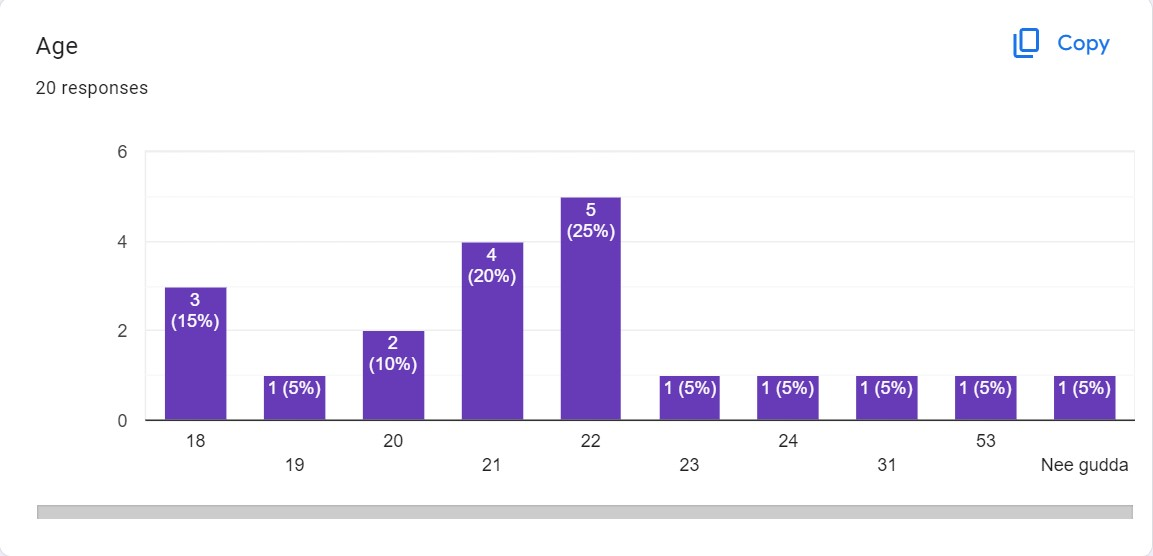
\includegraphics[scale=0.43]{Figures/responses-2.jpg}
    \caption{responses-2 \ref{fig::responses-2}}
    \label{fig::responses-2}
\end{figure}
\begin{figure}[H]
    \centering
    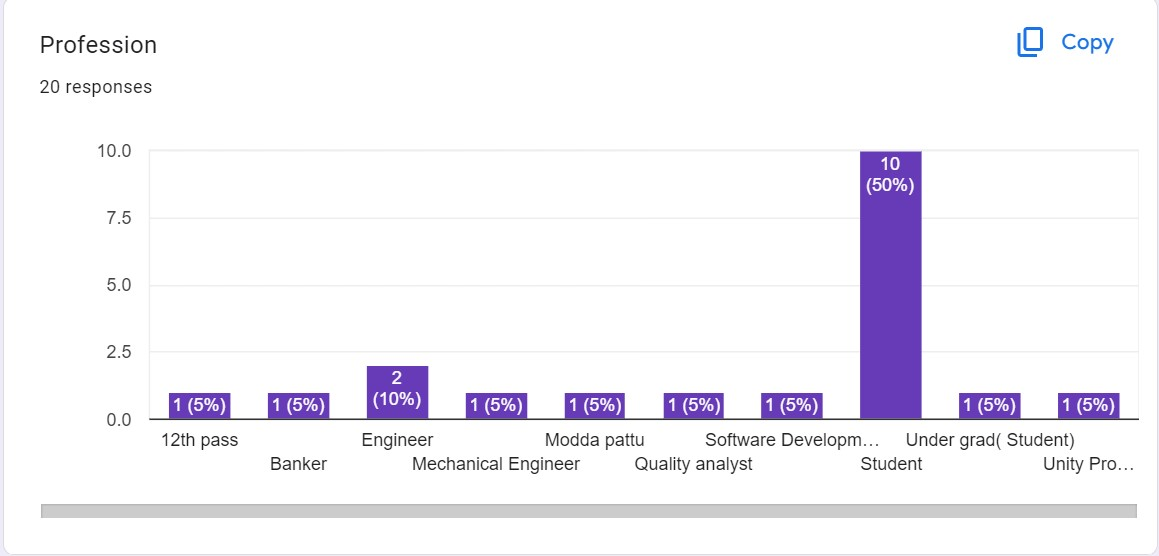
\includegraphics[scale=0.43]{Figures/responses-3.jpg}
    \caption{responses-3 \ref{fig::responses-3}}
    \label{fig::responses-3}
\end{figure}
\begin{figure}[H]
    \centering
    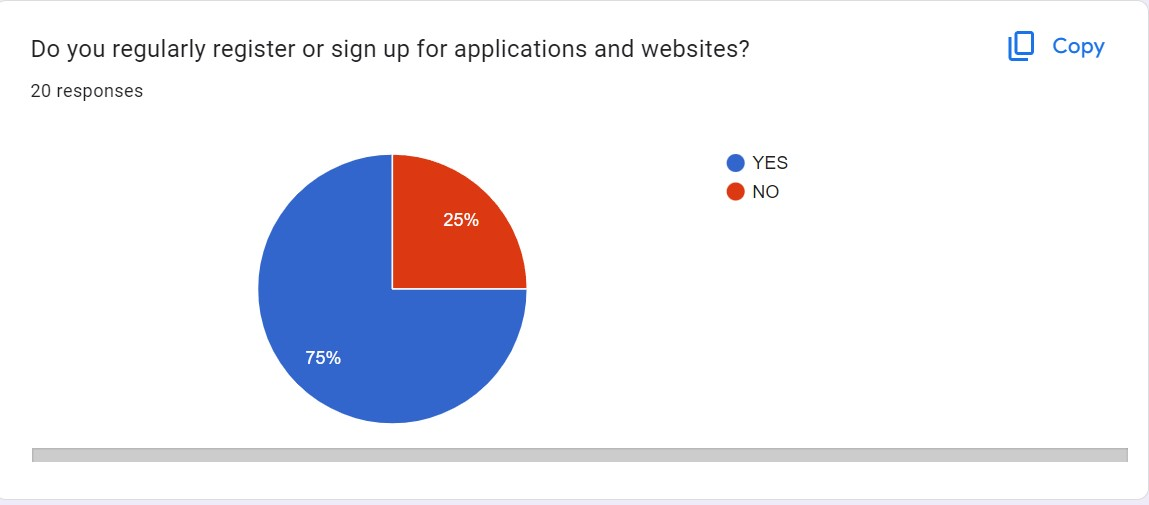
\includegraphics[scale=0.43]{Figures/responses-4.jpg}
    \caption{responses-4 \ref{fig::responses-4}}
    \label{fig::responses-4}
\end{figure}
\begin{figure}[H]
    \centering
    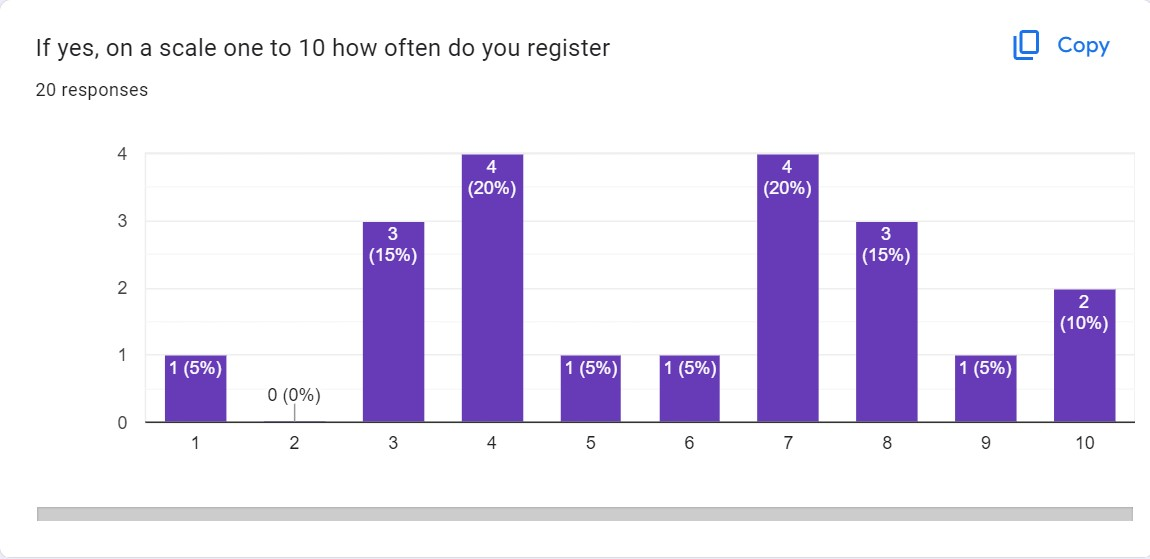
\includegraphics[scale=0.43]{Figures/responses-5.jpg}
    \caption{responses-5 \ref{fig::responses-5}}
    \label{fig::responses-5}
\end{figure}
\begin{figure}[H]
    \centering
    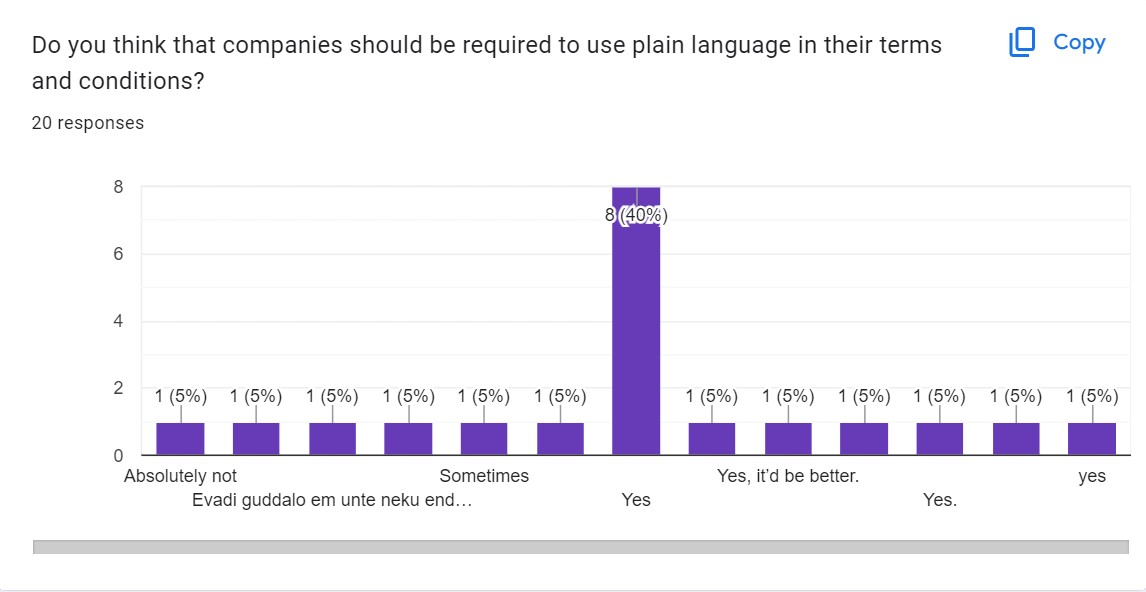
\includegraphics[scale=0.43]{Figures/responses-7.jpg}
    \caption{responses-7 \ref{fig::responses-7}}
    \label{fig::responses-7}
\end{figure}
\begin{figure}[H]
    \centering
    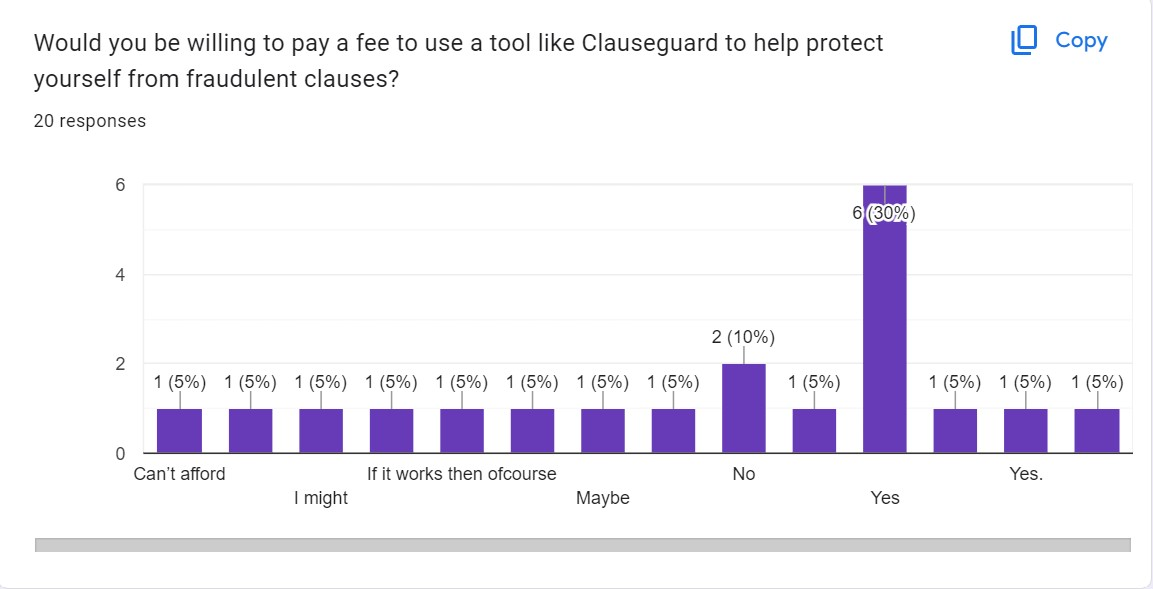
\includegraphics[scale=0.43]{Figures/responses-8.jpg}
    \caption{responses-8 \ref{fig::responses-8}}
    \label{fig::responses-8}
\end{figure}


    For Corporate lawyer, and law enforcement agency, we were unable to get any appointments for interviews. Hence, we asked chatgpt to act as a stakeholder. The conversations of those are given below: 

    \begin{itemize}
        \item Corporate Lawyer: 
    \end{itemize}


    
\section{ Jira:Project Management Tool \label{Jira Project Management Tool} }
Our team has used Jira which a project management tool to assign tasks and finish them on a weekly basis using sprints. 

\begin{figure}[H]
    \centering
    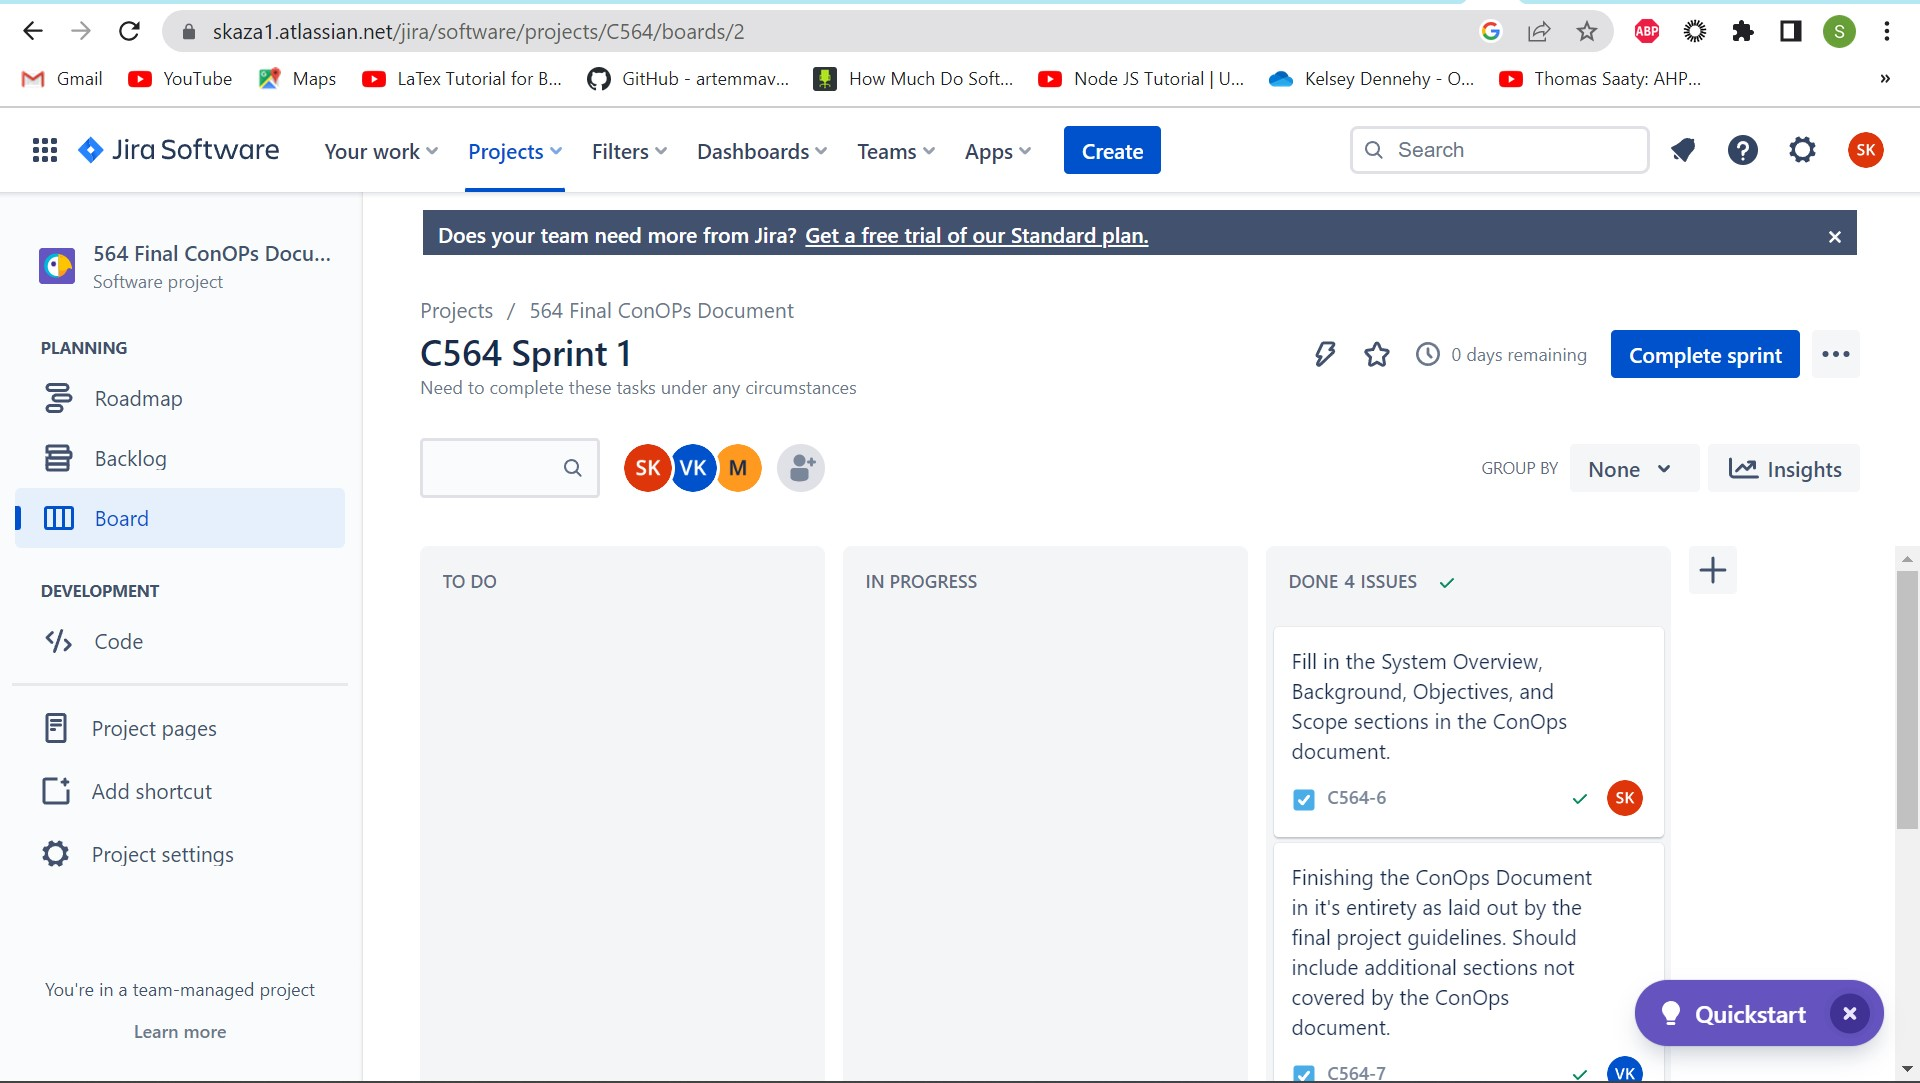
\includegraphics[scale=0.43]{Figures/Jira all completed tasks.jpg}
    \caption{Jira completion of tasks \ref{fig::Jira all completed tasks}}
    \label{fig::Jira all completed tasks}
\end{figure}


\begin{figure}[H]
    \centering
    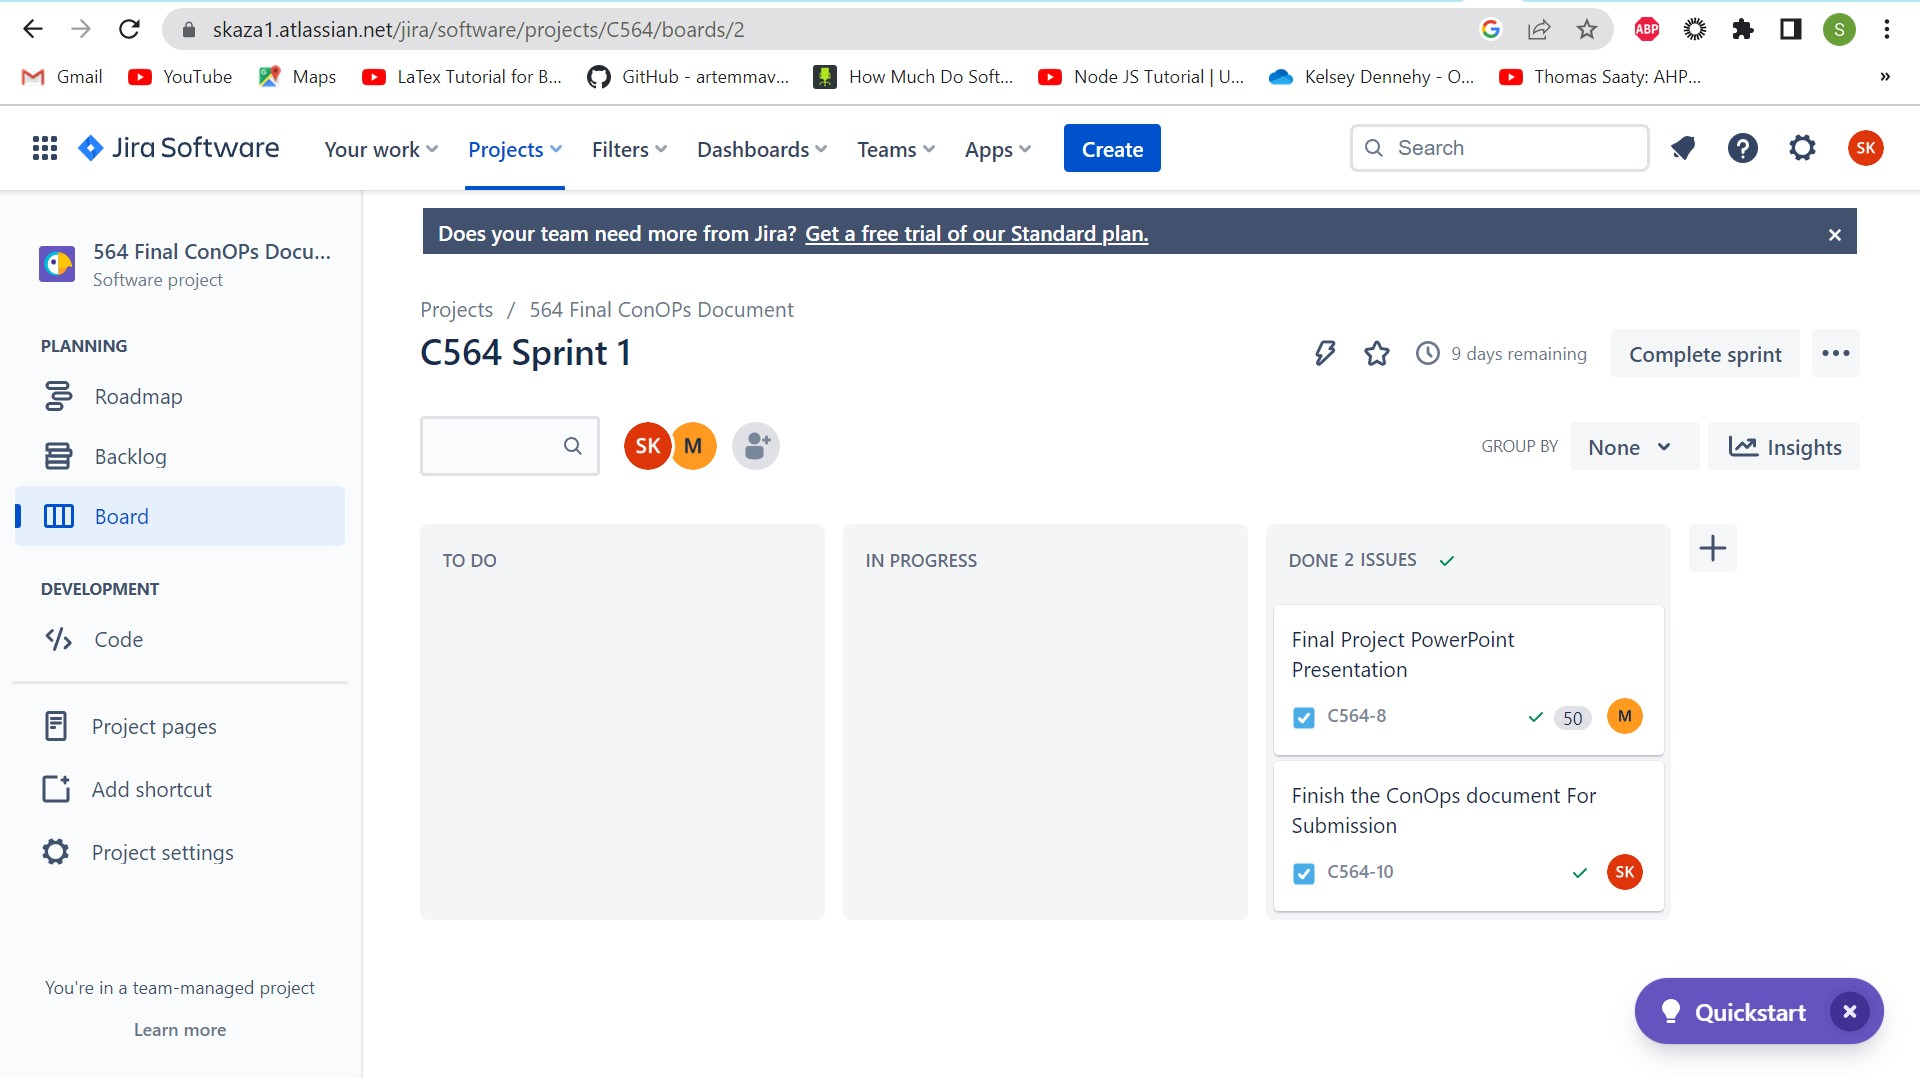
\includegraphics[scale=0.43]{Figures/All tasks completed.jpg}
    \caption{Jira completion of tasks \ref{fig::All tasks completed.jpg}}
    \label{fig::All tasks completed.jpg}
\end{figure}



\section{ Github:Version Tracking Tool \label{Github Version Tracking Tool} }

Our team used github for induce version changes and track previous versions. 

\begin{figure}[H]
    \centering
    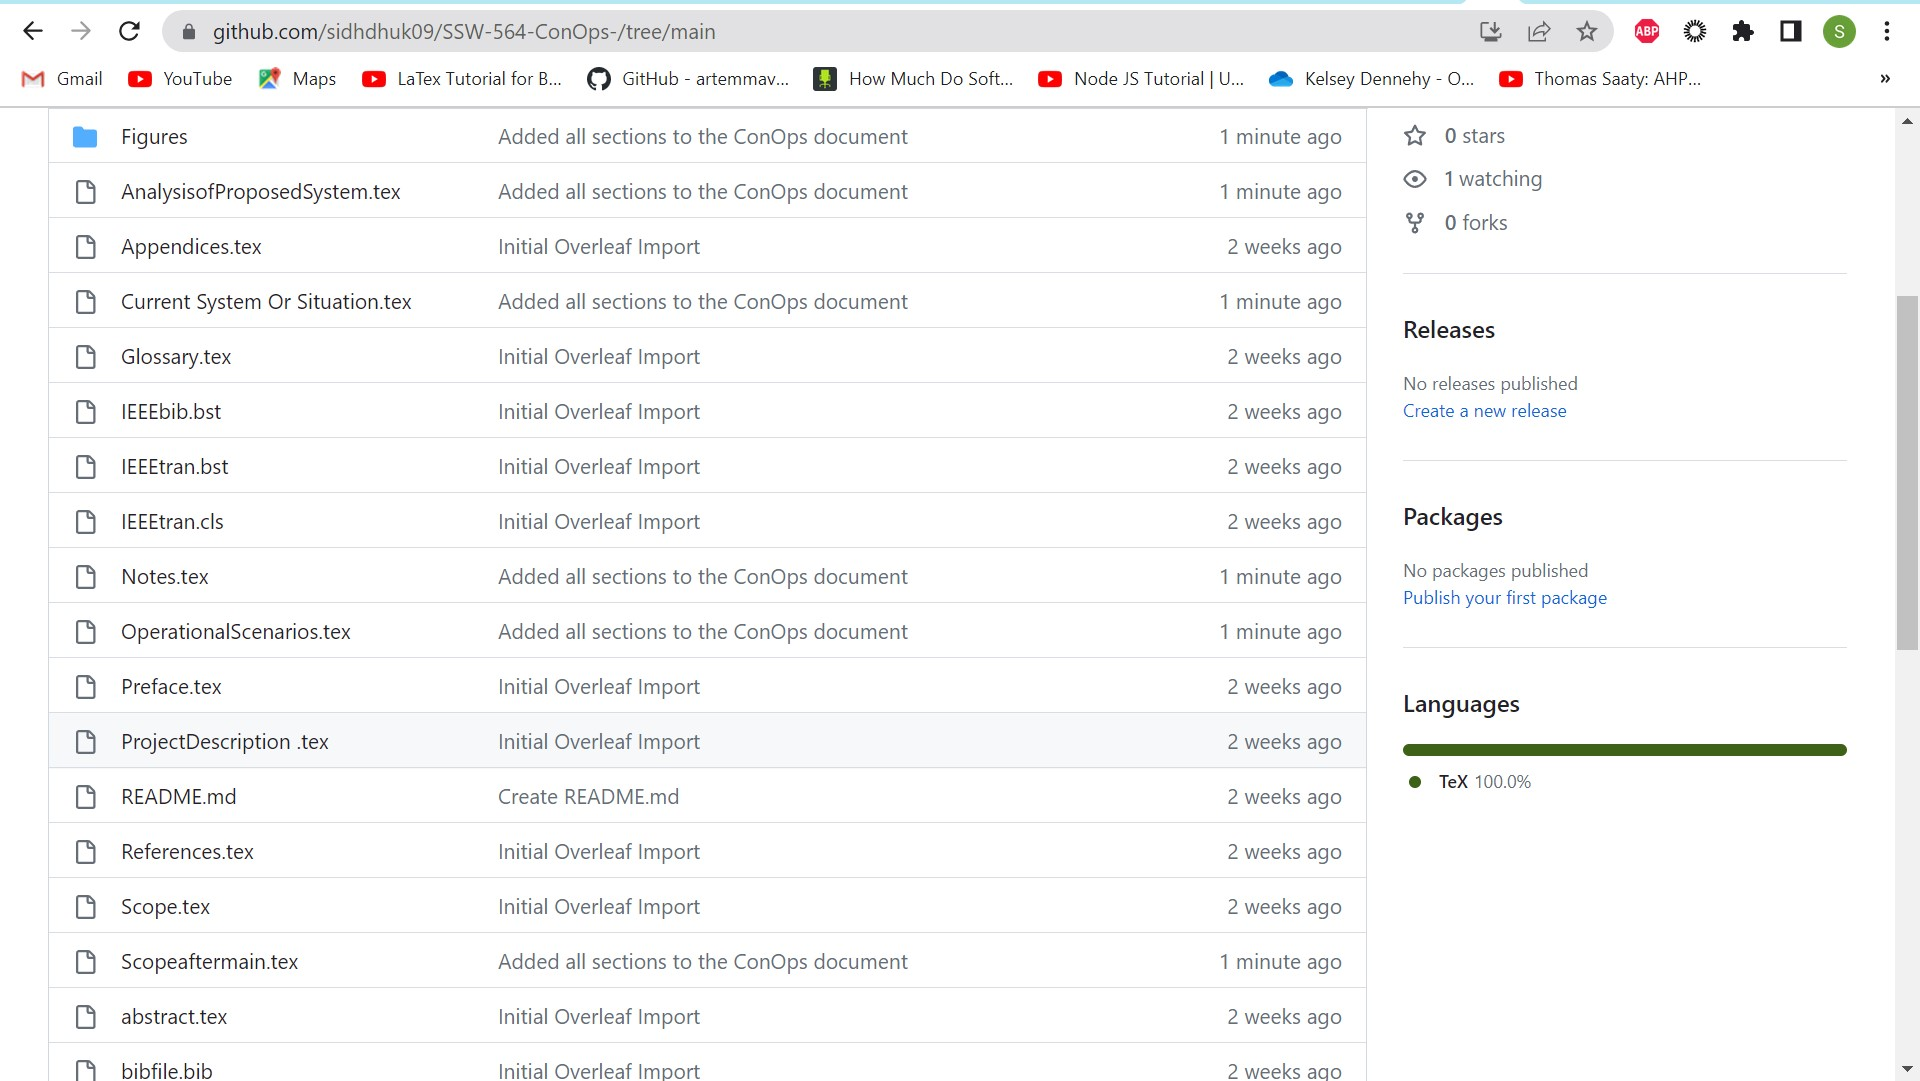
\includegraphics[scale=0.43]{Figures/github update-1.jpg}
    \caption{Jira completion of tasks \ref{fig::github update-1.jpg}}
    \label{fig::github update-1.jpg}
\end{figure}